% %
% main.tex
%

% notes = hide | show | only
\documentclass[xcolor=dvipsnames,dvip,notes=show,table]{beamer}

% Para crear una versión 'handout' (impresa)
%\documentclass[xcolor=pst,dvips,handout,notes=show]{beamer}

%
% cabeceras.tex
%

\usepackage[T1]{fontenc}

 \definecolor{ZurichBlue}{rgb}{.255,.41,.884}
 \beamertemplateshadingbackground{white!10}{white!10}
%\usepackage{beamerthemeWarsaw}

% \usepackage{longtable}
\usepackage{beamerthemeBoadilla}


%\usepackage{tikz,times}
\usetheme{boxes}
%\usepackage{handoutWithNotes}
\usepackage{pgfpages}
\pgfpagesuselayout{2 on 1}[a4paper,border shrink=5mm]


%\usecolortheme[named=OliveGreen]{structure} 
\setbeamertemplate{items}[ball] 
%\setbeamertemplate{blocks}[rounded][shadow=true] 
\setbeamertemplate{footline}[page number]
\addtocounter{framenumber}{-1}
%Handout



%\usepackage{beamertheme}
%\usepackage{beamerthemeshadow}
\useoutertheme[hooks]{tree}
 
% \setbeamertemplate{headline}[default] % The default is just an empty headline.
% \setbeamertemplate{headline}[infolines theme]
% \setbeamertemplate{headline}[miniframes theme]
% \setbeamertemplate{headline}[sidebar theme]
% \setbeamertemplate{headline}[smoothtree theme]
% \setbeamertemplate{headline}[smoothbars theme]
% \setbeamertemplate{headline}[tree]
\beamertemplatetransparentcovereddynamic
% spanish
\usepackage[spanish]{babel}
\usepackage[utf8]{inputenc}

% diagramas
%\usepackage{pst-eps,epstopdf}
\usepackage{pst-node}
%\usepackage{pst-all}
\usepackage{pst-blur}
%\usepackage{pst-tree}

% incrustaciones de código fuente
\usepackage{listings}

% matemáticas y símbolos
\usepackage{amsmath}
\usepackage{amssymb}
\usepackage[right]{eurosym}
\usepackage{ulem}

% colores
\usepackage{colortbl}

%\usepackage{algorithm2e}
%\usepackage{algorithm}
%\usepackage{algorithmic}

\lstset{language=[90]Fortran,
  basicstyle=\ttfamily,
  keywordstyle=\color{darkred},
  commentstyle=\color{green},
  frame=trBL,
  stringstyle=\color{violet},
  frameround=tttt,
  backgroundcolor=\color{lightyellow},
  morecomment=[l]{!\ }% Comment only with space after !
}


% 
% \lstset{%
%   language=Fortran,
% 	basicstyle=\footnotesize\sffamily,
% 	keywordstyle=\color{darkred}
%  	stringstyle=\color{violet}
%  	commentstyle=\color{blue}
%  	showspaces=false,
%  	showtabs=false,
%  	showstringspaces=false,
%  	frame=trBL,
%         frameround=tttt,
%         backgroundcolor=\color{lightyellow},
%  	extendedchars=true,
%  	numbers=none,
%         aboveskip=0.5cm,
%         belowskip=0.5cm,
%         xleftmargin=1cm,
%         xrightmargin=1cm,
% 	breaklines=true
% }
\definecolor{darkred}{rgb}{0.5, 0, 0}
\definecolor{violet}{rgb}{1, 0, 1}
\definecolor{lightyellow}{rgb}{1,1,0.8}


\usepackage{latexsym}
\usepackage{amsmath}
\usepackage{amssymb}
\usepackage{amsthm}

\usepackage{xspace}



\hyphenation{real}

\newrgbcolor{ColorEncabezadoTabla}{0.7 0.7 0.9}
\newrgbcolor{ColorFila1}{0.8 0.8 0.7}
\newrgbcolor{ColorFila2}{0.8 0.7 0.8}
\newrgbcolor{ColorTotal}{0.7 0.9 0.7}


% \usepackage{tikz,times}
% \usetikzlibrary{mindmap,backgrounds}



%%%%%%%%%%%%%%%%%%%%%%%%%%%%%%%%%%%%%%%%%%%%%%%%%%%%%%%%%%%%%%%%%%%%%%

\title[The RDFIndex approach | MTSR 2013]{Leveraging semantics to represent and compute quantitative indexes. \\ The RDFIndex approach.}
\author[Jose María Álvarez Rodríguez]{\textbf{Michalis Vafopoulos} (speaker) \\ and \\ \{Jose María Álvarez-Rodríguez, Patricia Ordoñez De Pablos and \\ Jose Emilio Labra-Gayo\}}
\institute{MTSR 2013 | 7th Metadata and Semantics Research Conference \\ Main Track}


\date{}

\begin{document}

\frame{
\titlepage

}


\frame{
\tableofcontents

}

\section{Introduction}

\frame{
  \frametitle{The Motivating example...} 
  
  
\begin{columns}[c] % the "c" option specifies center vertical alignment
\column{.5\textwidth} % column designated by a command


\begin{block}{Let's suppose that...}
 \begin{enumerate}
\item We want to create a ``Health index''...
\item ...to know which is the most ``healthy'' country.
\item ...to know which is the performance of the health expenditure .
\item ...to collect in just one value a set of indicators.
\item ...to make some new policy.
\end{enumerate}
\end{block}


\column{.5\textwidth}


\begin{figure}[htb]
\centering
	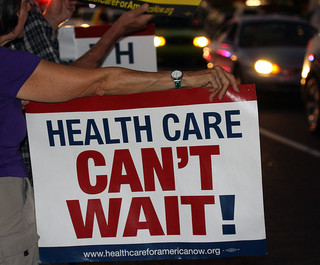
\includegraphics[width=4cm]{imgs/health}
%\caption{Modelo $5\star$ (W3C).}
\end{figure}

\end{columns}


}

\frame{
  \frametitle{The Motivating example...} 
  

\begin{block}{It is not a big deal because...}
 \begin{itemize}
\item We have the \textbf{``Health Index''} by an international network of physicians and researchers (\url{http://www.healthindex.com/}).
\item ...or the \textbf{``Health Index''} by the United Nations (\url{http://hdrstats.undp.org/en/indicators/72206.html}).
\item ...or the \textbf{``Ocean Health Index''} by an international collaborative effort (\url{http://www.oceanhealthindex.org/}).
\item ...or the indicators in the \textbf{World Bank} (\url{http://data.worldbank.org/topic/health}).
\item \ldots
\end{itemize}
\end{block}

}



\frame{
  \frametitle{The Motivating example...} 
 
   
\begin{exampleblock}{Benefits of using an index...}
 \begin{enumerate}
\item Creation of valuable data and information.
\item Generation of know-how to make some policy.
\item Re-use of a great effort and commitment by experts in some area.
\item Rank entities according to a quantitative value.
\item \ldots
\end{enumerate}
\end{exampleblock}

}

\frame{
  \frametitle{The Motivating example...} 
 
\scriptsize
\begin{alertblock}{Drawbacks of existing indexes...}<1->
 \begin{enumerate}
\item \textbf{Data heterogenity}: different datasources, formats and access protocols.
\item \textbf{Structure}: math models to aggregate some indicators that can change over time.
\item \textbf{Computation process}: observations are gathered and processed, \textit{somehow}, generating a final value.
\item \textbf{Documentation}: mutilingual and multicultural character of information.
\item \ldots
\end{enumerate}
\end{alertblock}

\begin{exampleblock}{..that imply the \textbf{necessity} of...}<2->
 \begin{enumerate}
\item \textbf{Accessing} \textbf{data} and information under a \textbf{common and shared data model}.
\item \textbf{Representing} the evolving \textbf{structure of the index}.
\item \textbf{Computing} the index to improve transparency.
\item Providing \textbf{context-aware documentation}: user-profile.
\item ... \textbf{Exploiting valuable data and metadata}.
\end{enumerate}
\end{exampleblock}

}


\frame{
  \frametitle{...but...Is it a common problem?} 
  

\begin{columns}[c] % the "c" option specifies center vertical alignment
\column{.5\textwidth} % column designated by a command


\begin{exampleblock}{...some indexes (per domain)...}
 \begin{enumerate}
\item Bibliography: the JCR and JSR, etc.
\item Government: the GDP, etc.
\item Web: the Webindex, etc.
\item Health: (the aforementioned ones).
\item Cloud: the CSC Cloud Usage Index, the VMWare index, the SMI index, etc.
\item ...to name a few per domain and creators.
\end{enumerate}
\end{exampleblock}


\column{.5\textwidth}


\begin{figure}[htb]
\centering
	
\includegraphics[width=5cm]{imgs/indexes}
%\caption{Modelo $5\star$ (W3C).}
\end{figure}

\end{columns}


}


\frame{
  \frametitle{A quantitative index is...}
  \begin{enumerate}
   \item It is technique to \textbf{collect in just one value} a set of indicators.
   \item It can be splitted into: index, component and indicator.
   \item An index is calculated by aggregating $n$ components using an \textbf{OWA operator}~\footnote{\textbf{Ordered weighted averaging} operator: $\sum_{i=1}^n  w_i a_i$, where \textbf{$w_i$} is the weight of the aggregated element \textbf{$a_i$}.}.
   \item A component is also calculated by aggregating $n$ indicators using an OWA operator.
   \item Observations are aligned to an indicator including some metadata such as: location, measure, value, etc.
  \end{enumerate}

  }
  
  
  
\frame{
  \frametitle{Graphical view of a quantitative index...}
\begin{figure}[htb]
\centering
	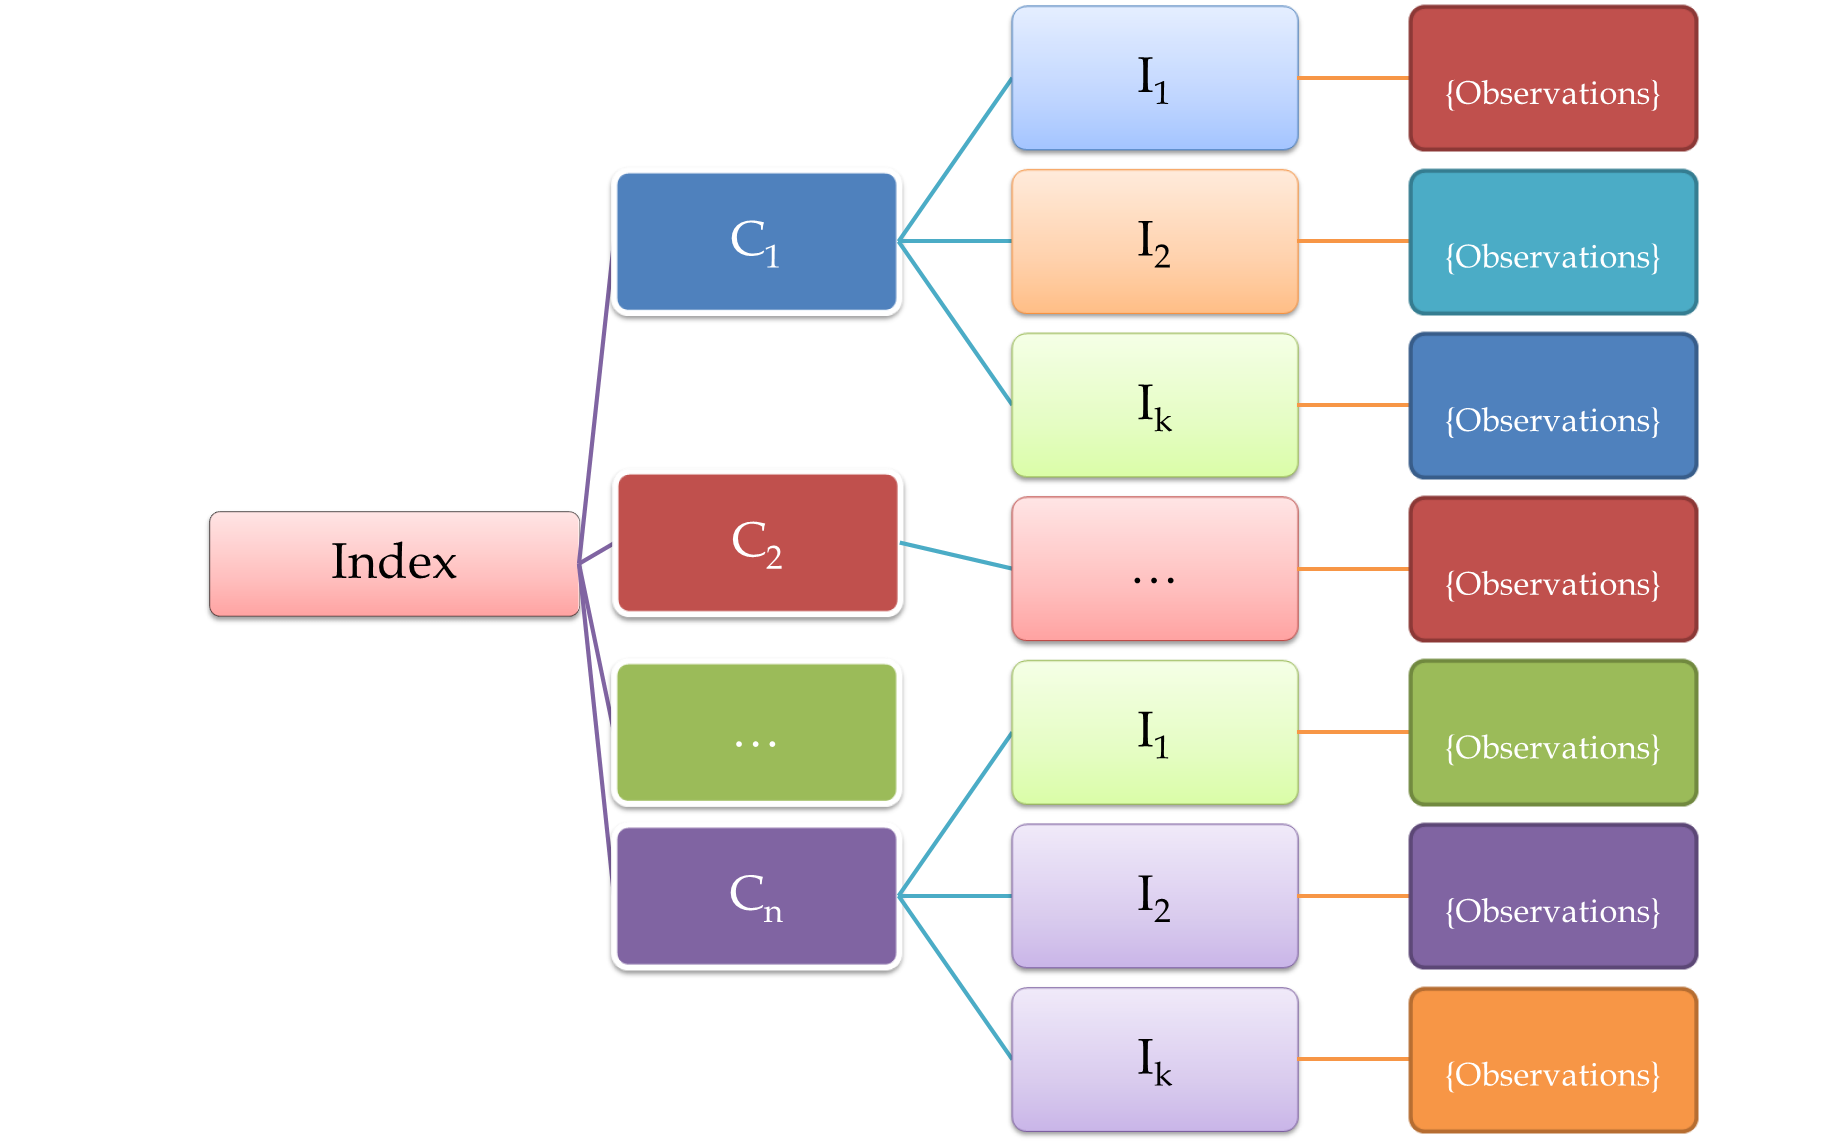
\includegraphics[width=10cm]{imgs/structure-index}
%\caption{Modelo $5\star$ (W3C).}
\end{figure}

  }
  
  
\section{Related Work}
\frame{
  \frametitle{Statistics and the Web of Data} 
  
\begin{block}{Vocabularies}<1->
  \begin{enumerate}
 \item The Statistical Core Vocabulary~\cite{scovo} (SCOVO), a former standard to describe statistical information in the Web of Data (2009).
 \item The RDF Data Cube Vocabulary~\cite{rdf-data-cube}, an adaptation of the ISO standard SDMX (Statistical Data and Metadata Exchange Vocabulary) (2013). 
 \item ``DDI-RDF discovery vocabulary. a metadata vocabulary for documenting research and survey data.'' (2013)~\cite{DDI2013} .
\end{enumerate}
\end{block}

  
 \begin{alertblock}{Preliminary evaluation...}<2->
  Existing RDF-based vocabularies enable us the possibility of modelling and representing statistical data.
 \end{alertblock}


}


\frame{
  \frametitle{Statistics and the Web of Data} 
\scriptsize
  \begin{exampleblock}{Statistics and Linked Data}<1->
  \begin{enumerate}
 \item ``Defining and Executing Assessment Tests on Linked Data for Statistical Analysis'' (2011)~\cite{DBLP:conf/semweb/ZapilkoM11}.
 \item ``Publishing Statistical Data on the Web'' (2012)~\cite{DBLP:journals/ijsc/SalasMBCMA12}.
 \item ``Publishing open statistical data: the Spanish census'' (2011)~\cite{DBLP:conf/dgo/FernandezMG11}.
 \item ``Publishing Statistical Data following the Linked Open Data Principles: The Web Index Project'' (2012)~\cite{webindexlod}.
 \item ``Linked Open Data Statistics: Collection and Exploitation'' (2013)~~\cite{DBLP:conf/kesw/ErmilovMLA13}.
 \item Some works in the ``RDF Validation Workshop 2013'' (\url{http://www.w3.org/2012/12/rdf-val/}).
\end{enumerate}
\end{exampleblock}


 
 \begin{alertblock}{Preliminary evaluation...}<2->
  All of the approaches are/were focused on data publishing/consumption...but...
  \begin{itemize}
   \item \textbf{Validation} of statistical data and/or structure...and
   \item the \textbf{Computation} process are still \textbf{open issues}.
  \end{itemize}

 \end{alertblock}


}

\section{Main Contributions}
\frame{
  \frametitle{Main Contributions} 
  
 \begin{exampleblock}{1-Representation}<1->
  A \textbf{high-level model on top of the RDF Data Cube Vocabulary} for representing quantitative indexes.
 \end{exampleblock}
 
 
 \begin{block}{2-Computation}<2->
  A \textbf{Java-SPARQL based processor} to exploit the meta-information, validate and compute the new index values.
 \end{block}

 }


\section{The RDFIndex approach}

\frame{
  \frametitle{Example: Building the ``The World Bank Naive Index''.} 
  \begin{itemize}
   \item Components: \textbf{``Aid Efectiveness''} ($c_1$) and \textbf{``Health''} ($c_2$).
   \item Indicators: \textbf{``Life Expectancy''} ($in_1$) and \textbf{``Health expenditure, total (\%) of GDP''} ($in_2$).
   \item The index, $i$, is calculated through the \textbf{ordered weighted averaging} (OWA) operator: $\sum_{i=1}^n  w_i c_i$, where $w_i$ is the weight of the component $c_i$
   \item All \textbf{observations} must be \textbf{normalized} using the \textit{z-score} before computing intermediate and final values for each indicator, component and index.
   \item It is necessary to populate the average age by country and year to create a new \textbf{``derivate'' indicator of ``Life Expectancy''} without the ``sex'' dimension.
  \end{itemize}
 
  }
  
\frame{
  \frametitle{Example of indicator observations from the WorldBank.} 
  
  \begin{table}[!htb]
\renewcommand{\arraystretch}{1.3}
\tiny
\begin{center}
\begin{tabular}{|p{4.5cm}|p{1cm}|p{2cm}|p{1cm}|p{1.5cm}|}
\hline
  \textbf{Description} & \textbf{Year} & \textbf{Country} & \textbf{Value} & \textbf{Status} \\  \hline
  Life Expectancy Male & 2010 & Spain & $79$ & Normal \\ \hline
  Life Expectancy Male & 2011 & Spain & $79$ & Normal\\ \hline
  Life Expectancy Female & 2010 & Spain & $85$ & Normal\\ \hline
  Life Expectancy Female & 2011 & Spain & $85$ & Normal\\ \hline
  Life Expectancy Male & 2010 & Greece & $78$ & Normal\\ \hline
  Life Expectancy Male & 2011 & Greece & $79$ & Normal\\ \hline
  Life Expectancy Female & 2010 & Greece & $83$ & Normal\\ \hline
  Life Expectancy Female & 2011 & Greece & $83$ & Normal\\ \hline
  Health expenditure, total (\% of GDP) & 2010 & Spain & $74.2$ & Normal\\ \hline
  Health expenditure, total (\% of GDP) & 2011 & Spain & $73.6$ & Normal\\ \hline
  Health expenditure, total (\% of GDP) & 2010 & Spain & $61.5$ & Normal\\ \hline
  Health expenditure, total (\% of GDP) & 2011 & Spain & $61.2$ & Normal\\ \hline
  \hline
  \end{tabular}
   \label{tab:example-wb}
  \end{center}	 
\end{table} 


}

\frame{
  \frametitle{Representing and computing data with the RDFIndex (summary)}
  
  \begin{exampleblock}{Steps}
   \begin{enumerate}
    \item Define the structure and computation of the index with the RDFIndex vocabulary.
    \item Run the Java SPARQL based processor:
    \begin{itemize}
    \item Load the RDFIndex ontology to have access to common definitions.
    \item Create a kind of Abstract Syntax Tree (AST) containing the defined meta-data (our index).
    \item Validate the structure with an AST Walker (structure and RDF Data Cube normalization).
    \item Create the SPARQL queries to compute the index (another AST walker).
    \item Load the observations and run the SPARQL queries to generate new observations.
    \end{itemize}
 \end{enumerate}
\end{exampleblock}

}


\frame{
  \frametitle{Graphical view of the RDFIndex workflow...}
\begin{figure}[htb]
\centering
	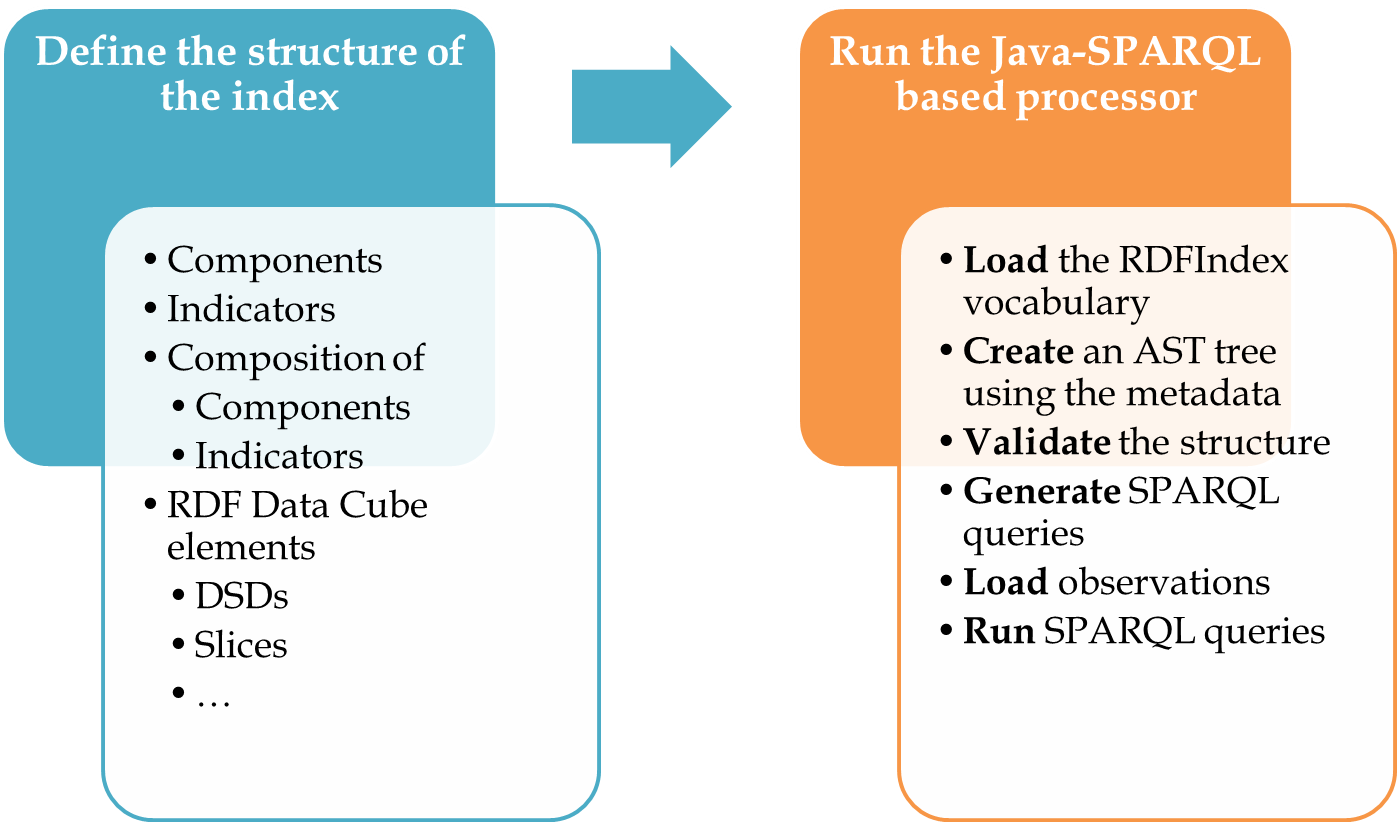
\includegraphics[width=10cm]{imgs/index-flow}
%\caption{Modelo $5\star$ (W3C).}
\end{figure}

  }
  
  
  

\frame{
  \frametitle{Underlying definitions}

\scriptsize
\begin{block}{Observation-$o$}
It is a tuple $\{v,m,s\}$, where $v$ is a numerical value for the measure $m$ with an status $s$ that belongs to 
only one dataset of observations $O$. 
\end{block}


\begin{exampleblock}{Dataset-$q$}
It is a tuple $\{O,m,D,A,T\}$ where $O$ is a set of observations for only one measure $m$ that is described under 
a set of dimensions $D$ and a set of annotations $A$. Additionally, some attributes can be defined in the set $T$ for structure enrichment. 
\end{exampleblock}


\begin{alertblock}{Aggregated dataset-$aq$}
It is an aggregation of $n$ datasets $q_i$ (identified by the set $Q$) which set of observations $O$ is derivate by applying 
an OWA operator $p$ to the observations $O_{q_i}$. 
\end{alertblock}

}

\frame{
  \frametitle {Scope and Consequences}

\scriptsize

\begin{exampleblock}{Necessary condition for the computation process}
An aggregated dataset $aq$ defined by means of the set of dimensions $D_{aq}$ can be computed iif 
$\forall q_j \in Q: D_{aq} \subseteq D_{q_j}$. Furthermore the OWA operator $p$ can only aggregate values belonging to the same measure $m$.
\end{exampleblock}


\begin{itemize}
 \item The set of dimensions $D$, annotations $A$ and attributes $T$ for a given dataset $Q$ is always the same with the aim of describing all observations under 
 the same context.
 \item An index $i$ and a component $c$ are aggregated datasets. Nevertheless this restriction is relaxed if observations can be directly mapped to 
 these elements without any computation process.
 \item An indicator $in$ can be both dataset or aggregated dataset.
 \item All elements in definitions must be uniquely identified. 
 \item An aggregated dataset is also a dataset.
\end{itemize}

}



\frame{
  \frametitle{Mapping the RDFIndex to the RDF Data Cube Vocabulary} 
  
 \begin{table}[!htb]
\renewcommand{\arraystretch}{1.3}
\tiny
\begin{center}
\begin{tabular}{|p{2cm}||p{3.8cm}|p{3.5cm}|}
\hline
  \textbf{Concept} & \textbf{Vocabulary element} &  \textbf{Comments}  \\  \hline
   Observation $o$ & \texttt{qb:Observation} &  Enrichment through annotations\\ \hline
   Numerical value $v$ & \texttt{xsd:double} & Restriction to numerical values  \\ \hline
   Measure $m$ & \texttt{qb:MeasureProperty} \texttt{sdmx-measure:obsValue} & Restriction to one measure \\ \hline
   Status $s$ & \texttt{sdmx-concept:obsStatus} & Defined by the SDMX-RDF vocabulary\\ \hline
   Dataset $q$ & \texttt{qb:dataSet} and \texttt{qb:qb:DataStructureDefinition} &  Metadata of the \texttt{qb:dataSet}\\ \hline
   Dimension $d_i \in D$ & \texttt{qb:DimensionProperty} & Context of observations \\ \hline
   Annotation $a_i \in A$ & \texttt{owl:AnnotationProperty} &  Intensive use of Dublin Core\\ \hline
   Attribute $at_i \in T$ & \texttt{qb:AttributeProperty} & Link to existing datasets such as DBPedia \\ \hline
   OWA operator $p$ &  SPARQL 1.1 aggregation operators & Other extensions depend on the RDF repository \\ \hline
   Index, Component and Indicator & \texttt{skos:Concept} & SKOS taxonomy (logical structure) \\ \hline
  \hline
  \end{tabular}
 % \caption{Summary of mappings between the index definition and the RDF Data Cube Vocabulary.}
  \label{index-to-rdf}
  \end{center}
\end{table} 

}

\begin{frame}[fragile]
\frametitle{Example of the ``World Bank Naive index'' structure in RDF.}
\begin{figure}[!ht]
\begin{lstlisting}[language=XML,basicstyle=\tiny]  
@prefix rdfindex:  <http://purl.org/rdfindex/ontology/> .
@prefix rdfindex-wb:  <http://purl.org/rdfindex/wb/resource/> .
@prefix rdfindex-wbont:  <http://purl.org/rdfindex/wb/ontology/> .

rdfindex-wb:TheWorldBankNaiveIndex 
  a rdfindex:Index;
  rdfs:label "The World Bank Naive Index"@en;
  rdfindex:type rdfindex:Quantitative;
  rdfindex:aggregates [ 		
    rdfindex:aggregation-operator rdfindex:OWA;
    rdfindex:part-of [
      rdfindex:dataset rdfindex-wb:AidEffectiveness; 
      rdfindex:weight 0.4];
    rdfindex:part-of [rdfindex:dataset rdfindex-wb:Health; 
      rdfindex:weight 0.6];
  ];
  #More meta-data properties...
  qb:structure 	rdfindex-wb:TheWorldBankNaiveIndexDSD ; .
  
rdfindex-wb:TheWorldBankNaiveIndexDSD 
  a qb:DataStructureDefinition;  
  qb:component    
  [qb:dimension rdfindex-wbont:ref-area],
  [qb:dimension rdfindex-wbont:ref-year],
  [qb:measure   rdfindex:value],
  [qb:attribute sdmx-attribute:unitMeasure];
  #More meta-data properties...
  .
\end{lstlisting}
 \label{fig:results-rdf-index}
\end{figure}
\end{frame}


\begin{frame}[fragile]
\frametitle{SPARQL template for building aggregated observations.}
\begin{figure}[!ht]
\begin{lstlisting}[language=SQL,basicstyle=\scriptsize,mathescape]  
SELECT ($d_i \in D$) [(sum(?w*?measure) as ?newvalue) | OWA(?measure)]
WHERE{
  $q$ rdfindex:aggregates ?parts.
  ?parts rdfindex:part-of ?partof.
  ?partof rdfindex:dataset $q_i$ .
  FILTER($?partof \in Q$).  
  ?observation rdf:type qb:Observation.
  ?part rdfindex:weight ?defaultw.     
  OPTIONAL {?partof rdfindex:weight ?aggregationw.}.
  BIND (if( BOUND(?aggregationw), ?aggregationw, ?defaultw) AS ?w)
  ?observation $m$ ?measure . 
  ?observation ?dim ?dimRef. 
  FILTER ($?dim  \in D$).
}GROUP BY ($d_i \in D$)
\end{lstlisting}
 \label{fig:results-rdf-sparql-template}
\end{figure}
\end{frame}



\begin{frame}[fragile]
\frametitle{Example of generated SPARQL query.}
\begin{figure}[!ht]
\begin{lstlisting}[language=SQL,basicstyle=\scriptsize]  
prefix rdfindex:  <http://purl.org/rdfindex/ontology/> 
SELECT ?dim0 ?dim1 ( sum(?w*?measure) as ?newvalue) 
WHERE{ 
  rdfindex-wb:TheWorldBankNaiveIndex  
  rdfindex:aggregates ?parts.
  ?parts rdfindex:part-of ?partof.
  ?partof rdfindex:dataset ?part .
  FILTER ((?part =rdfindex-wb:AidEffectiveness) || 
	  (?part =rdfindex-wb:Health)). 
  ?observation qb:dataSet ?part . 
  ?part rdfindex:weight ?defaultw.        
  OPTIONAL {?partof rdfindex:weight ?aggregationw.}.
  BIND (if( BOUND(?aggregationw), ?aggregationw, ?defaultw) AS ?w)
  ?observation rdfindex:value ?measure . 
  ?observation rdfindex-wbont:ref-area ?dim0. 
  ?observation rdfindex-wbont:ref-year ?dim1. 
} GROUP BY ?dim0 ?dim1 
\end{lstlisting}
 
\end{figure}
\end{frame}




\begin{frame}[fragile]
\frametitle{Partial example of a populated observation for ``The World Bank Naive Index''.}
\begin{figure}[!ht]
\begin{lstlisting}[language=SQL,basicstyle=\scriptsize]  
rdfindex-wb:o6808100851579
      a       qb:observation ;
      qb:dataSet rdfindex-wb:TheWorldBankNaiveIndex  ;
      rdfindex-wbont:ref-area dbpedia-res:Spain ;
      rdfindex-wbont:ref-year
	<http://reference.data.gov.uk/id/
	gregorian-interval/2010-01-01T00:00:00/P1Y> ;
      ...
      #rdfs:{label,comment} {literal};
      #dcterms:{issued, date, contributor, author, 
      #publisher, identifier} 
      #{resource, literal};
      rdfindex:md5-hash "6cdda76088cd161d766809d6a78d35f6";
      sdmx-concept:obsStatus
              sdmx-code:obsStatus-E;
      rdfindex:value "0.707"^^xsd:double .
\end{lstlisting}
 
\end{figure}
\end{frame}




\frame{
  \frametitle{Evolution: joint effort between RDFIndex and Computex}
  \scriptsize
  \begin{block}{Computex}
   \begin{enumerate}
    \item Vocabulary for statistical computations.
    \item Extends RDF Data Cube.
    \item Ontology at: \url{http://purl.org/weso/computex}.
    \item Data and structure validation using SPARQL Queries.
    \item Some terms:
    \begin{itemize}
     \item \texttt{cex:Concept}
    \item \texttt{cex:Indicator}
    \item \texttt{cex:Computation}
    \item \texttt{cex:WeightSchema}
    \item \texttt{qb:Observation}
    \end{itemize}
    \item Learn more: \url{http://computex.herokuapp.com/}
   \end{enumerate}
   \end{block}

  \begin{exampleblock}{Preliminary Evaluation...}
   Similar approaches that have been merged between July and September, 2013.
  \end{exampleblock}


}


\frame{
  \frametitle{Demo of the RDFIndex/Computex...}
\begin{figure}[htb]
\centering
	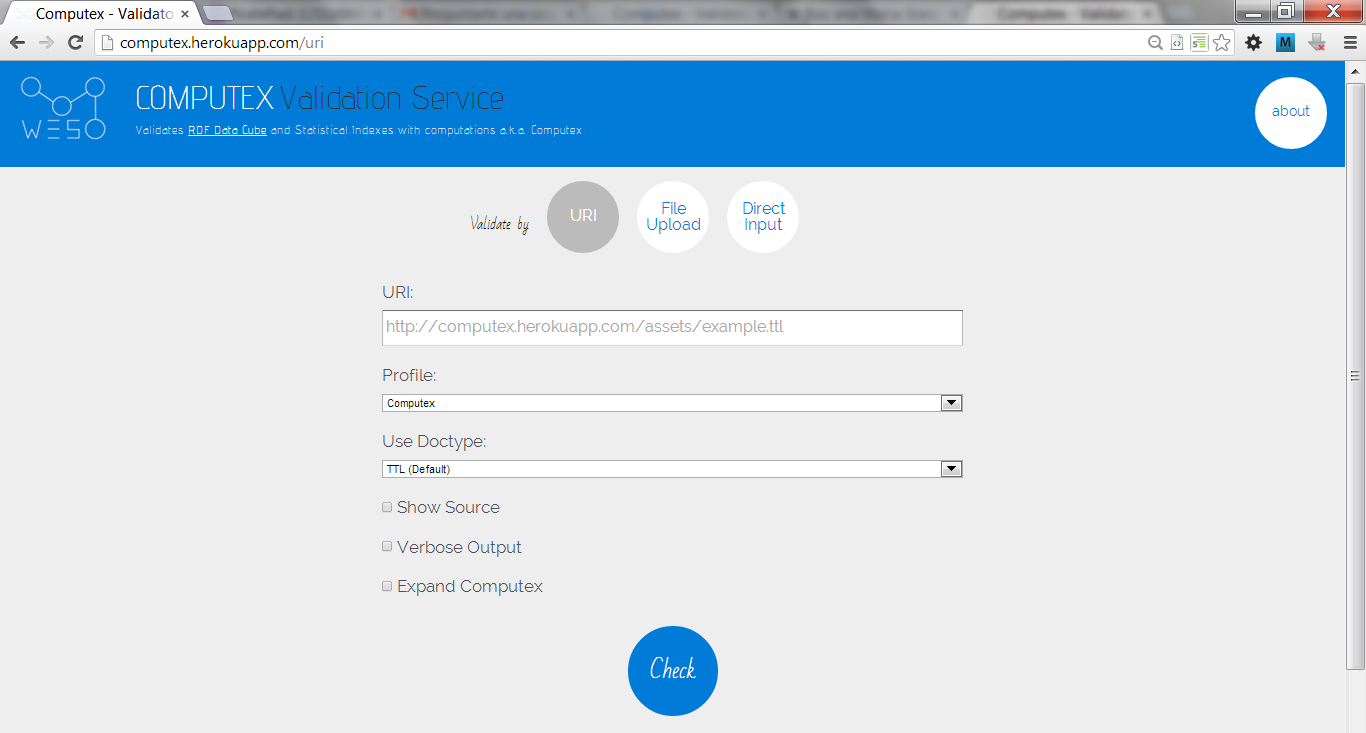
\includegraphics[width=10cm]{imgs/computex}
%\caption{Modelo $5\star$ (W3C).}
\end{figure}

\url{http://computex.herokuapp.com/}
  }
  
  
\frame{
  \frametitle{On-going working examples}
  \scriptsize
  \begin{block}{The Cloud Index}<1->
   \begin{itemize}
    \item Compilation of \textbf{Key Performance Indicators} for cloud services.
    \item Creation of a Cloud Index to measure \textbf{Quality of Service} of cloud providers.
    \item Funded by: the RELATE-ITN (FP7-PEOPLE-2010-ITN, 264840) project and developed in the subproject 
    \textbf{``Quality Management in Service-based Systems and Cloud Applications''}.
    \item Demo: \url{http://cloudindex-doc.herokuapp.com/}
   \end{itemize}

  \end{block}

  \begin{exampleblock}{The Web Index 2012 and 2013}<2->
   \begin{itemize}
    \item Compilation of several indicators (85) from \textbf{61 countries} (100 in 2013).
    \item Creation of the Web Index to measure the web impact over the world.
    \item Funded by: The Webfoundation.
    \item Demo: \url{http://thewebindex.org}
   \end{itemize}
  \end{exampleblock}

}




\section{Evaluation and Discussion}


\frame{
  \frametitle{Advantages} 
 \begin{exampleblock}{Data Sources}<1->
  Data management applying the Linked Data principles.
 \end{exampleblock}

 \begin{block}{Structure}<2->
Automatic validation and verfication of the structure and metadata of quantitative indexes.
 \end{block}

 
 
 \begin{alertblock}{Computation process}<3->
A native approach using SPARQL queries that can help to boost transparency.
 \end{alertblock}

 
  \begin{exampleblock}{Documentation}<4->
Implicit multilingual and multicultural support.
 \end{exampleblock}

 
 
 
 }

\frame{
  \frametitle{Detailed advantages (I)} 
  
   
   
\begin{table}[!htb]
\renewcommand{\arraystretch}{1.3}
\tiny
\begin{center}
\begin{tabular}{|p{2cm}|p{8.5cm}|}
\hline
  \textbf{Feature} & \textbf{Main advantages}  \\  \hline
  Data sources  & \begin{itemize}
		      \item Common and shared data model, RDF.
		      \item Description of data providers (provenance and trust).
		      \item A formal query language to query data, SPARQL.
		      \item Use of Internet protocols, HTTP.
		      \item Data enrichment and validation (domain and range).
		      \item Unique identification of entities, concepts, etc. through (HTTP) URIs.
		      \item Possibility of publishing new data under the aforementioned characteristics.
		      \item Standardization and integration of data sources.
		    \end{itemize} \\ \hline  
  Structure & \begin{itemize}
                  \item Meta-description of index structure (validation).
                  \item Re-use of existing semantic web vocabularies.
                  \item Re-use of existing datasets to enrich meta-data.
                  \item Context-aware definitions.
                  \item Underlying logic formalism.                  
                  \item Orthogonal and flexible.                 
                 \end{itemize} \\ \hline       
  \hline
  \end{tabular}
  \end{center}
\end{table} 



}



\frame{
  \frametitle{Detailed advantages (II)} 
  
   
\begin{table}[!htb]
\renewcommand{\arraystretch}{1.3}
\tiny
\begin{center}
\begin{tabular}{|p{2cm}|p{8.5cm}|}
\hline
  Computation process & \begin{itemize}
                  \item Meta-description of datasets aggregation.
                  \item Validation of composed datasets.
                  \item OWA operators support.
                  \item Direct translation to SPARQL queries.  
                 \end{itemize} \\ \hline
  Documentation & \begin{itemize}
                  \item Multilingual support to describe datasets, etc.
                  \item Easy generation with existing tools.                
                 \end{itemize} \\ \hline      
                 
                 Cross-Domain Features & \begin{itemize}
                  \item Separation of concerns and responsibilities: data and meta-data (structure and computation).
                  \item Standardization (put in action specs from organisms such as W3C).
                  \item Declarative and adaptive approach.
                  \item Non-vendor lock-in (format, access and computation).
                  \item Integration, Interoperability and Transparency.
                  \item Align to existing trend (data management: quality and filtering).
                  \item Easy integration with third-party services such as visualization.
                  \item Contribution to the Web of Data.
                 \end{itemize} \\ \hline        
       
  \hline
  \end{tabular}
  \end{center}
\end{table} 



}



\frame{
  \frametitle{Restrictions} 
  
  
 \begin{alertblock}{SPARQL 1.1 support}<1->
\begin{enumerate}
 \item Some built-in functions are not standardized:
 \begin{itemize}
  \item Example: \texttt{z-score} employs standard deviation. 
  \item It requires built-in function: \texttt{sqrt} (only available in some SPARQL implementations).
 \end{itemize}
 \item Ranking of values is not obvious: 
  \begin{itemize} \item \texttt{GROUP\_CONCAT} 
    \item Check a value against all the other values.
     \item ...neither solution is efficient.
   \end{itemize}
\end{enumerate}
\end{alertblock}
 
 \begin{block}{Limitations of the RDFIndex expressivity}<2->
  The working examples show its applicability but some lack of terms/relationships should be expected.
 \end{block}

}


\section{Conclusions and Future Work}

\frame{
  \frametitle{Conclusions} 
}


\frame{
  \frametitle{Future Work} 
}

\frame{
    
  \begin{figure}[!htb]
\centering
 
\includegraphics[width=9cm]{imgs/thanks}
\end{figure}


}

\section{Metadata and Information}



\frame{
  \frametitle{Acknowledgements} 
\begin{figure}[!htb]
\centering
 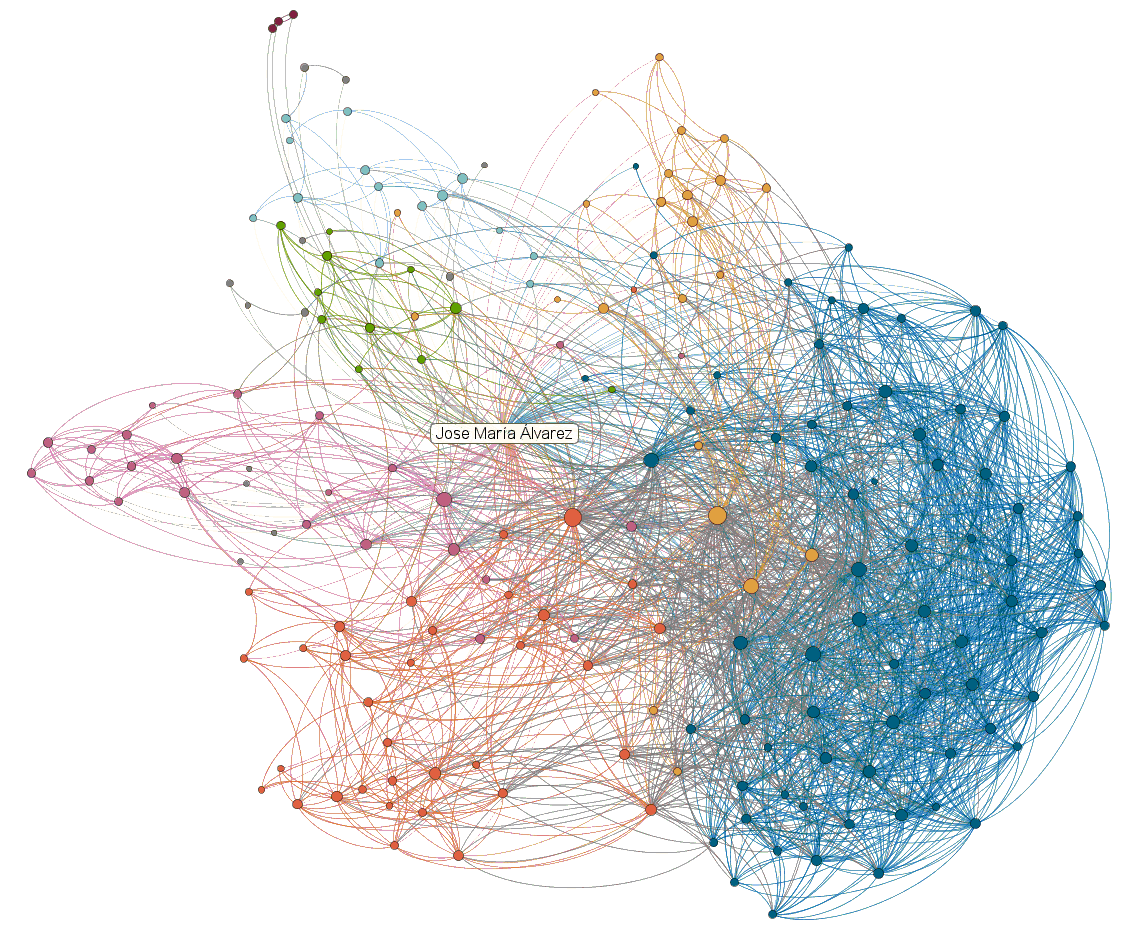
\includegraphics[width=9cm]{imgs/linkedin}
\end{figure}
}


\frame{
  \frametitle{Contact} 
}

\frame{
  \frametitle{Credits} 
}

\frame{
  \frametitle{Resources} 
}

\appendix
\section*{References}
\bibliographystyle{abbrv}
\tiny
\bibliography{references}


% %%%%%%%%%%%%%%%%%%%%%%%%%%%%%%%%%%%%%%%%%%%%%%%%%%%%%%%%%%%%%%%%%%%%%%

\normalsize

\frame{
\titlepage

}


\end{document}
